\section{Suddivisione del lavoro e prospetto orario}
Ogni componente del gruppo dovrà ricoprire ogni ruolo almeno una volta nel corso del \glossaryItem{progetto}.
Durante lo stesso periodo un componente può ricoprire più ruoli, a condizione che le mansioni previste non vadano in conflitto tra loro; ad esempio non è ammessa la \glossaryItem{verifica} del proprio lavoro.
Segue il prospetto orario suddiviso per periodi e totale. \\

Nell'intestazione utilizzata per le tabelle di questo capitolo sono state impiegate \textbf{abbreviazioni} per i nomi dei ruoli.
Di seguito viene riportato il loro significato, \textbf{nell'ordine in cui sono utilizzate} nell'intestazione:
\begin{itemize}
\item Amm.: \textit{Amministratore};
\item Ana.: \textit{Analista};
\item Pgt.: \textit{Progettista};
\item Pgr.: \textit{Programmatore};
\item Res.: \textit{Responsabile};
\item Ver.: \textit{Verificatore}.
\end{itemize}

%-----------------------------------------------------------------------------------------------------
%-------------------------------------- ANALISI ------------------------------------------------------
%-----------------------------------------------------------------------------------------------------
\pagebreak
\subsection{Analisi}
Nel periodo di \textit{Analisi} ciascun componente dovrà rivestire i seguenti ruoli:

\begin{table}[H]
\begin{tabular}{lccccccc}
\toprule
    \textbf{Nome}  & \multicolumn{6}{c}{\textbf{Ore per ruolo}} & \textbf{Ore totali} \\
     & Amm. & Ana. & Pgt. & Pgr. & Res. & Ver. & \\
    \midrule
    
	   Andrea Mantovani & 15 & 0 & 0 & 0 & 10 & 0 & 25 \\
	     Davide Polonio & 18 & 0 & 4 & 0 & 0 & 0 & 22 \\
	      Davide Rigoni & 0 & 14 & 0 & 0 & 5 & 9 & 28 \\
	   Emanuele Carraro & 0 & 12 & 0 & 0 & 0 & 9 & 21 \\
	Giovanni Mazzocchin & 0 & 12 & 0 & 0 & 0 & 9 & 21 \\
	        Luca Bianco & 0 & 12 & 0 & 0 & 0 & 9 & 21 \\
	    Matteo Di Pirro & 0 & 0 & 4 & 0 & 18 & 0 & 22 \\
    %totale ore: 160 
    
    \bottomrule
\end{tabular}
\caption{Ore per componente, periodo di \textit{Analisi}}
\end{table}


I valori in tabella sono riassunti nel seguente grafico: \\ 

    \begin{figure}[H]
      \begin{center}
        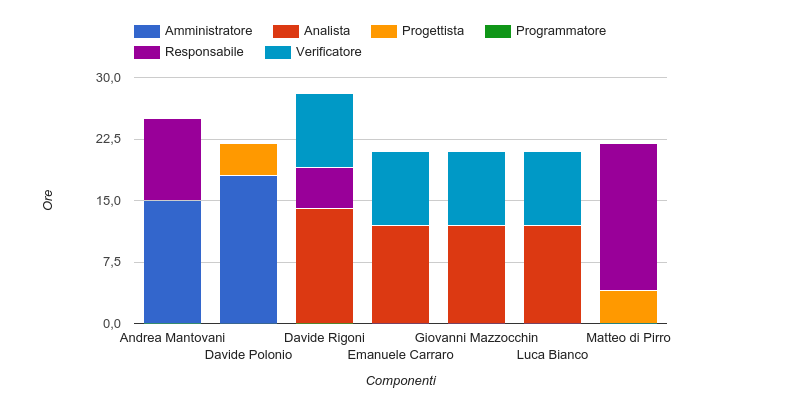
\includegraphics[width=15cm]{res/img/suddivisioneRuoloProspettoOrario/orePerComponenteAnalisi.png}
      \caption{Ore per componente, periodo di \textit{Analisi}}
      \end{center} 
    \end{figure}    
    
Si fa notare che le ore sopra indicate non sono incluse nelle 105 ore rappresentanti il tetto massimo di ore somministrabili a ciascun componente.


%-----------------------------------------------------------------------------------------------------
%-------------------------------------- ANALISI  MIGLIORAMENTI ---------------------------------------
%-----------------------------------------------------------------------------------------------------
\pagebreak
\subsection{Analisi Miglioramenti}
Nel periodo di \textit{Analisi Miglioramenti} ciascun componente dovrà rivestire i seguenti ruoli:

\begin{table}[H]
\begin{tabular}{lccccccc}
\toprule
    \textbf{Nome}  & \multicolumn{6}{c}{\textbf{Ore per ruolo}} & \textbf{Ore totali} \\
     & Amm. & Ana. & Pgt. & Pgr. & Res. & Ver. & \\
    \midrule
    
	   Andrea Mantovani & 0 & 0 & 3 & 0 & 0 & 0 & 3 \\
	     Davide Polonio & 0 & 0 & 0 & 0 & 1 & 0 & 1 \\
	      Davide Rigoni & 0 & 0 & 0 & 0 & 0 & 0 & 0 \\
	   Emanuele Carraro & 11 & 0 & 0 & 0 & 0 & 0 & 11 \\
	Giovanni Mazzocchin & 0 & 0 & 0 & 0 & 0 & 5 & 5 \\
	        Luca Bianco & 0 & 0 & 0 & 0 & 0 & 6 & 6 \\
	    Matteo Di Pirro & 0 & 4 & 0 & 0 & 0 & 0 & 4 \\
    %totale ore: 30 
    
    \bottomrule
\end{tabular}
\caption{Ore per componente, periodo di \textit{Analisi Miglioramenti}}
\end{table}


I valori in tabella sono riassunti nel seguente grafico: \\ 

    \begin{figure}[H]
      \begin{center}
        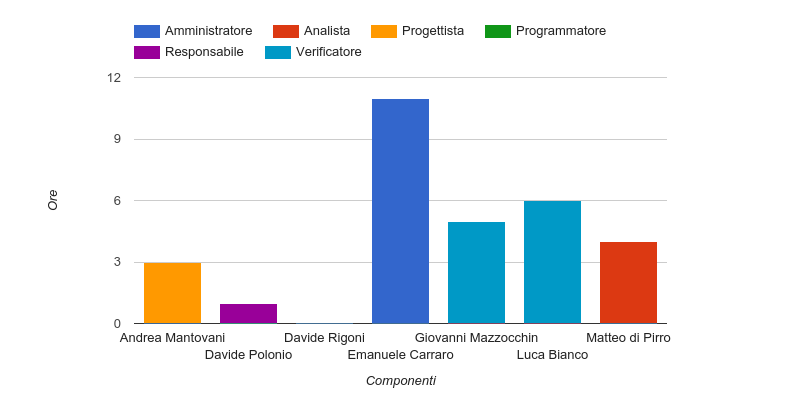
\includegraphics[width=15cm]{res/img/suddivisioneRuoloProspettoOrario/orePerComponenteAnalisiMiglioramenti.png}
      \caption{Ore per componente, periodo di \textit{Analisi Miglioramenti}}
      \end{center} 
    \end{figure}    

%-----------------------------------------------------------------------------------------------------
%-------------------------------------- PROGETTAZIONE ARCHITETTURALE ---------------------------------
%-----------------------------------------------------------------------------------------------------
\pagebreak
\subsection{Progettazione Architetturale}
Nel periodo di \textit{Progettazione Architetturale} ciascun componente dovrà rivestire i seguenti ruoli:

\begin{table}[H]
\begin{tabular}{lccccccc}
\toprule
    \textbf{Nome}  & \multicolumn{6}{c}{\textbf{Ore per ruolo}} & \textbf{Ore totali} \\
     & Amm. & Ana. & Pgt. & Pgr. & Res. & Ver. & \\
    \midrule
    
	   Andrea Mantovani & 0 & 3 & 16 & 0 & 0 & 14 & 33 \\
	     Davide Polonio & 0 & 0 & 20 & 0 & 0 & 12 & 32 \\
	      Davide Rigoni & 8 & 0 & 15 & 0 & 0 & 10 & 33 \\
	   Emanuele Carraro & 0 & 0 & 25 & 0 & 0 & 10 & 35 \\
	Giovanni Mazzocchin & 0 & 0 & 20 & 0 & 2 & 8 & 30 \\
	        Luca Bianco & 0 & 0 & 22 & 0 & 0 & 10 & 32 \\
	    Matteo Di Pirro & 0 & 0 & 23 & 0 & 0 & 10 & 33 \\
           %totale ore: 228
    
    \bottomrule
\end{tabular}
\caption{Ore per componente, periodo di \textit{Progettazione Architetturale}}
\end{table}

I valori in tabella sono riassunti nel seguente grafico: \\ 

    \begin{figure}[H]
      \begin{center}
        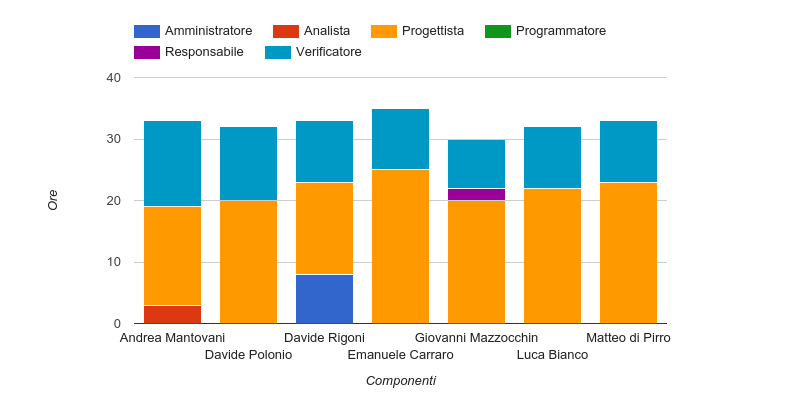
\includegraphics[width=15cm]{res/img/suddivisioneRuoloProspettoOrario/orePerComponenteProgettazioneArchitetturale.png}
      \caption{Ore per componente, periodo di \textit{Progettazione Architetturale}}
      \end{center} 
    \end{figure}    
    
    
    
    
%-----------------------------------------------------------------------------------------------------
%-------------------------------------- PROGETTAZIONE DI DETTAGLIO E CODIFICA ------------------------
%-----------------------------------------------------------------------------------------------------
\pagebreak
\subsection{Progettazione di Dettaglio e Codifica}
Nel periodo di \textit{Progettazione di Dettaglio e Codifica} ciascun componente dovrà rivestire i seguenti ruoli:

\begin{table}[H]
\begin{tabular}{lccccccc}
\toprule
    \textbf{Nome}  & \multicolumn{6}{c}{\textbf{Ore per ruolo}} & \textbf{Ore totali} \\
     & Amm. & Ana. & Pgt. & Pgr. & Res. & Ver. & \\
    \midrule
    
	   Andrea Mantovani & 0 & 0 & 20 & 21 & 0 & 12 & 53 \\
	     Davide Polonio & 0 & 3 & 30 & 23 & 0 & 0 & 56 \\
	      Davide Rigoni & 0 & 0 & 20 & 23 & 0 & 14 & 57 \\
	   Emanuele Carraro & 0 & 0 & 0 & 25 & 3 & 16 & 44 \\
	Giovanni Mazzocchin & 25 & 0 & 15 & 15 & 0 & 0 & 55 \\
	        Luca Bianco & 25 & 0 & 15 & 16 & 0 & 0 & 56 \\
	    Matteo Di Pirro & 0 & 0 & 20 & 18 & 0 & 12 & 50 \\
           %totale ore: 371
    
    
    \bottomrule
\end{tabular}
\caption{Ore per componente, periodo di \textit{Progettazione di dettaglio e codifica}}
\end{table}

I valori in tabella sono riassunti nel seguente grafico: \\ 

    \begin{figure}[H]
      \begin{center}
        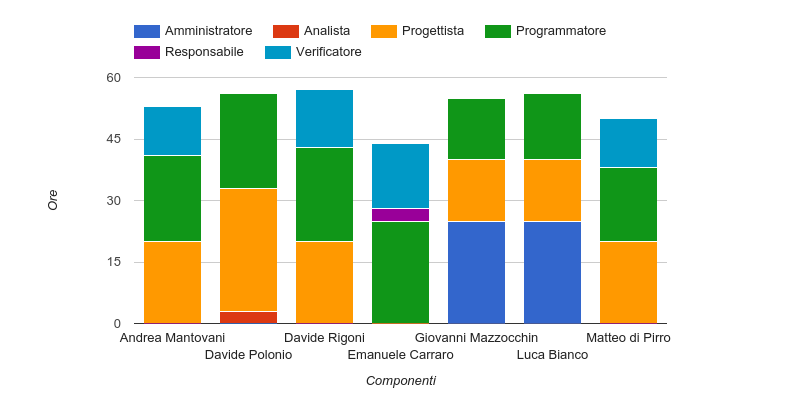
\includegraphics[width=15cm]{res/img/suddivisioneRuoloProspettoOrario/orePerComponenteProgettazioneDettaglioCodifica.png}
      \caption{Ore per componente, periodo di \textit{Progettazione di Dettaglio e Codifica}}
      \end{center} 
    \end{figure}    
    
    
    
%-----------------------------------------------------------------------------------------------------
%-------------------------------------- VALIDAZIONE ---------------------------------------
%-----------------------------------------------------------------------------------------------------
\pagebreak
\subsection{Validazione}
Nel periodo di \glossaryItem{Validazione} ciascun componente dovrà rivestire i seguenti ruoli:

\begin{table}[H]
\begin{tabular}{lccccccc}
\toprule
    \textbf{Nome}  & \multicolumn{6}{c}{\textbf{Ore per ruolo}} & \textbf{Ore totali} \\
     & Amm. & Ana. & Pgt. & Pgr. & Res. & Ver. & \\
    \midrule
    
	   Andrea Mantovani & 0 & 0 & 6 & 5 & 0 & 5 & 16 \\
	     Davide Polonio & 0 & 0 & 6 & 0 & 0 & 10 & 16 \\
	      Davide Rigoni & 0 & 0 & 0 & 0 & 0 & 15 & 15 \\
	   Emanuele Carraro & 0 & 0 & 0 & 0 & 0 & 15 & 15 \\
	Giovanni Mazzocchin & 0 & 0 & 0 & 0 & 0 & 15 & 15 \\
	        Luca Bianco & 0 & 0 & 0 & 0 & 6 & 5 & 11 \\
	    Matteo Di Pirro & 13 & 0 & 0 & 0 & 0 & 5 & 18 \\
           %totale ore: 106 --> totale 895 -160 = 735
    
    \bottomrule
\end{tabular}
\caption{Ore per componente, periodo di \glossaryItem{Validazione}}
\end{table}

I valori in tabella sono riassunti nel seguente grafico: \\ 

    \begin{figure}[H]
      \begin{center}
        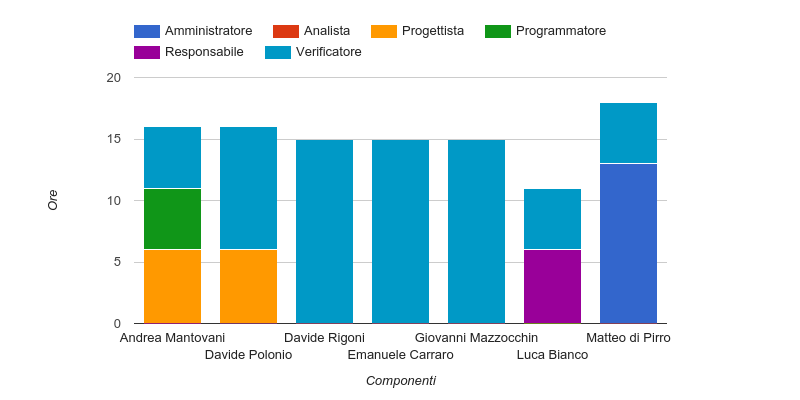
\includegraphics[width=15cm]{res/img/suddivisioneRuoloProspettoOrario/orePerComponenteValidazione.png}
      \caption{Ore per componente, periodo di \glossaryItem{Validazione}}
      \end{center} 
    \end{figure}    
   
    
    
%-----------------------------------------------------------------------------------------------------
%-------------------------------------- TOTALE -------------------------------------------------------
%-----------------------------------------------------------------------------------------------------
\pagebreak
\subsection{Totale}
Il totale delle ore, comprensive delle ore di \textit{Analisi} che saranno fornite da ciascun membro
del gruppo nel corso dell’intero \glossaryItem{progetto} sono le seguenti:

\begin{table}[H]
\begin{tabular}{lccccccc}
\toprule
    \textbf{Nome}  & \multicolumn{6}{c}{\textbf{Ore per ruolo}} & \textbf{Ore totali} \\
     & Amm. & Ana. & Pgt. & Pgr. & Res. & Ver. & \\
    \midrule
   
	   Andrea Mantovani & 15 & 3 & 45 & 26 & 10 & 31 & 130 \\
	     Davide Polonio & 18 & 3 & 60 & 23 & 1 & 22 & 127 \\
	      Davide Rigoni & 8 & 14 & 35 & 23 & 5 & 48 & 133 \\
	   Emanuele Carraro & 11 & 12 & 25 & 30 & 3 & 50 & 131 \\
	Giovanni Mazzocchin & 25 & 12 & 35 & 15 & 2 & 37 & 126 \\ 
	        Luca Bianco & 25 & 12 & 37 & 16 & 6 & 30 & 126 \\ 
	    Matteo Di Pirro & 13 & 4 & 47 & 18 & 18 & 27 & 127 \\ 
   			%totale ore: 895
   
    \bottomrule
\end{tabular}
\caption{Ore per componente totali, incluso il periodo di \textit{Analisi}}
\end{table}

I valori in tabella sono riassunti nel seguente grafico: \\ 

    \begin{figure}[H]
      \begin{center}
        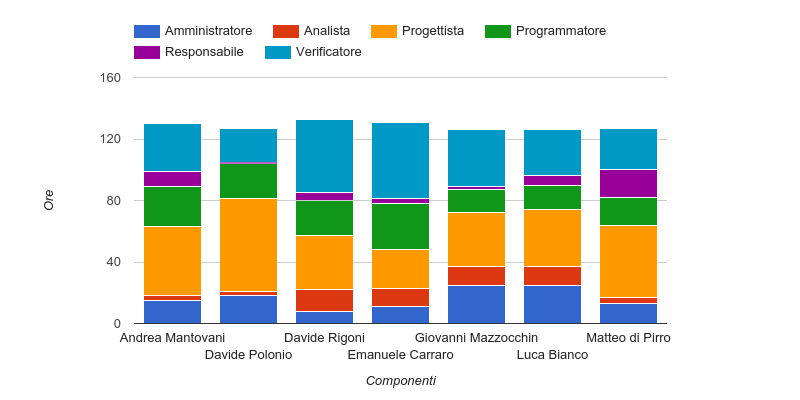
\includegraphics[width=15cm]{res/img/suddivisioneRuoloProspettoOrario/orePerComponenteTotaliConAnalisi.png}
      \caption{Ore per componente totali, incluso il periodo di \textit{Analisi}}
      \end{center} 
    \end{figure}    
    

Quelle esenti dall'\textit{Analisi}:

\begin{table}[H]
\begin{tabular}{lccccccc}
\toprule
    \textbf{Nome}  & \multicolumn{6}{c}{\textbf{Ore per ruolo}} & \textbf{Ore totali} \\
     & Amm. & Ana. & Pgt. & Pgr. & Res. & Ver. & \\
    \midrule
   
	   Andrea Mantovani & 0 & 3 & 45 & 26 & 0 & 31 & 105 \\
	     Davide Polonio & 0 & 3 & 56 & 23 & 1 & 22 & 105 \\
	      Davide Rigoni & 8 & 0 & 35 & 23 & 0 & 39 & 105 \\
	   Emanuele Carraro & 11 & 0 & 25 & 25 & 3 & 41 & 105 \\
	Giovanni Mazzocchin & 25 & 0 & 35 & 15 & 2 & 28 & 105 \\
	        Luca Bianco & 25 & 0 & 37 & 16 & 6 & 21 & 105 \\
	    Matteo Di Pirro & 13 & 4 & 43 & 18 & 0 & 27 & 105 \\
   			%totale ore: 735
   
    \bottomrule
\end{tabular}
\caption{Ore per componente totali, incluso il periodo di \textit{Analisi}}
\end{table}

I valori in tabella sono riassunti nel seguente grafico: \\ 

    \begin{figure}[H]
      \begin{center}
        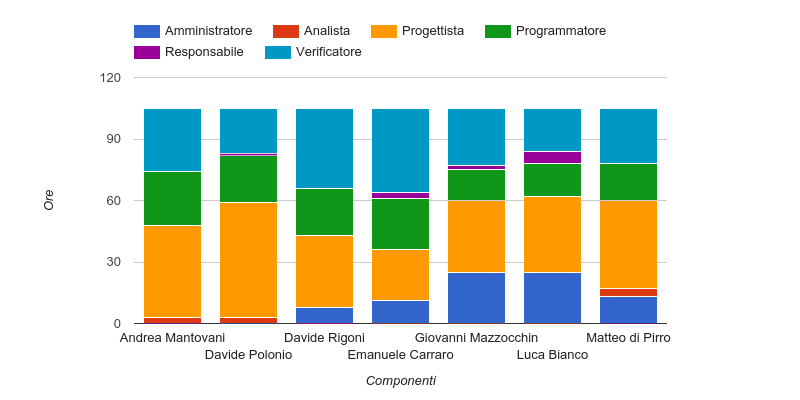
\includegraphics[width=15cm]{res/img/suddivisioneRuoloProspettoOrario/orePerComponenteTotaliSenzaAnalisi.png}
      \caption{Ore per componente totali, incluso il periodo di \textit{Analisi}}
      \end{center} 
    \end{figure}    
    
    
